%%%%%%%%%%%%%%%%%%%%%%%%%%%%%%%%%%%%%%%%%%%%%%%%%%%%%%%%%%%%%%%
% Karo Takhleeq Phase 2 Report
% Smart Course Registration Chrome Extension
% User Validation & Initial MVP Planning
%%%%%%%%%%%%%%%%%%%%%%%%%%%%%%%%%%%%%%%%%%%%%%%%%%%%%%%%%%%%%%%

\documentclass[11pt, a4paper]{article}

\usepackage[utf8]{inputenc}
\usepackage[T1]{fontenc}
\usepackage{lmodern}
\usepackage[margin=0.9in]{geometry}
\usepackage{graphicx}
\usepackage{xcolor}
\usepackage{tikz}
\usepackage{pgfplots}
\usepackage{tcolorbox}
\usepackage{enumitem}
\usepackage{fontawesome5}
\usepackage{hyperref}
\usepackage{fancyhdr}
\usepackage{titlesec}
\usepackage{booktabs}
\usepackage{tabularx}
\usepackage{multicol}

\usetikzlibrary{shapes.geometric, arrows.meta, positioning, shadows, calc, patterns, decorations.pathreplacing}
\pgfplotsset{compat=1.18}

% Colors
\definecolor{primaryblue}{RGB}{59, 130, 246}
\definecolor{successgreen}{RGB}{16, 185, 129}
\definecolor{warningyellow}{RGB}{245, 158, 11}
\definecolor{dangerred}{RGB}{239, 68, 68}
\definecolor{textdark}{RGB}{30, 41, 59}
\definecolor{textgray}{RGB}{100, 116, 139}
\definecolor{bglight}{RGB}{248, 250, 252}

% tcolorbox styles
\tcbuselibrary{skins, breakable}

\newtcolorbox{insightbox}[1]{
    enhanced, colback=successgreen!8, colframe=successgreen,
    fonttitle=\bfseries, title={#1}, boxrule=0pt, leftrule=4pt,
    arc=4pt, left=10pt, right=10pt, top=8pt, bottom=8pt,
    before skip=10pt, after skip=10pt
}

\newtcolorbox{questionbox}[1]{
    enhanced, colback=primaryblue!8, colframe=primaryblue,
    fonttitle=\bfseries\color{white}, title={\faIcon{question-circle} #1},
    boxrule=0pt, leftrule=4pt, arc=4pt, colbacktitle=primaryblue,
    attach boxed title to top left={yshift=-2mm, xshift=5mm},
    boxed title style={arc=2pt, boxrule=0pt},
    before skip=12pt, after skip=12pt
}

\newtcolorbox{featurebox}{
    enhanced, colback=white, colframe=primaryblue!50,
    boxrule=1pt, arc=8pt, left=10pt, right=10pt,
    drop shadow={opacity=0.1}, before skip=8pt, after skip=8pt
}

% Header/Footer
\pagestyle{fancy}
\fancyhf{}
\fancyhead[L]{\small\color{textgray}\textit{Karo Takhleeq 2026}}
\fancyhead[R]{\small\color{textgray}\textit{Phase 2 Report}}
\fancyfoot[C]{\thepage}
\renewcommand{\headrulewidth}{0.5pt}

% Section formatting
\titleformat{\section}{\Large\bfseries\color{primaryblue}}{\thesection.}{0.5em}{}[\titlerule]
\titleformat{\subsection}{\large\bfseries\color{textdark}}{\thesubsection}{0.5em}{}

\hypersetup{colorlinks=true, linkcolor=primaryblue, urlcolor=primaryblue}

%%%%%%%%%%%%%%%%%%%%%%%%%%%%%%%%%%%%%%%%%%%%%%%%%%%%%%%%%%%%%%%
\begin{document}

% Title Page
\begin{titlepage}
\begin{tikzpicture}[remember picture, overlay]
    \fill[primaryblue] (current page.north west) rectangle ([yshift=-4cm]current page.north east);
    \node[white, font=\Huge\bfseries] at ([yshift=-2cm]current page.north) {KARO TAKHLEEQ 2026};
\end{tikzpicture}

\vspace*{4cm}
\begin{center}
    {\color{warningyellow}\Large\bfseries --- Phase 2 Submission ---}
    
    \vspace{1.5cm}
    {\Huge\bfseries\color{textdark} User Validation \&}\\[0.3cm]
    {\Huge\bfseries\color{primaryblue} Initial MVP Planning}
    
    \vspace{1cm}
    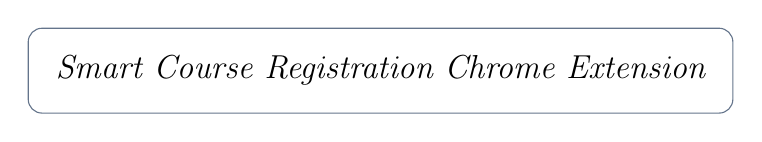
\begin{tikzpicture}
        \node[draw=textgray, rounded corners=5pt, inner sep=10pt, font=\large\itshape] 
            {Smart Course Registration Chrome Extension};
    \end{tikzpicture}
    
    \vspace{2cm}
    
    % Survey Stats Summary
    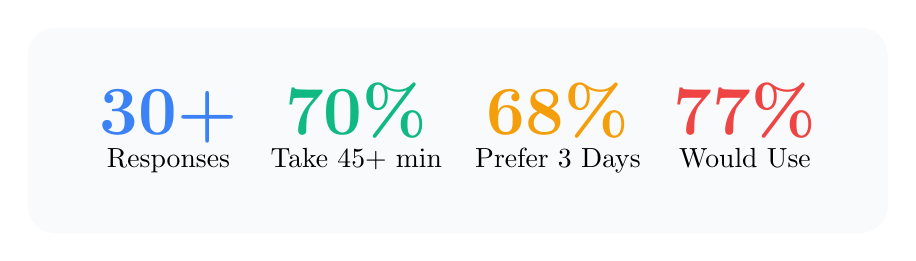
\begin{tikzpicture}
        \node[fill=bglight, rounded corners=10pt, inner sep=20pt] {
            \begin{tabular}{cccc}
                \textbf{\color{primaryblue}\Huge 30+} & 
                \textbf{\color{successgreen}\Huge 70\%} & 
                \textbf{\color{warningyellow}\Huge 68\%} & 
                \textbf{\color{dangerred}\Huge 77\%} \\
                Responses & Take 45+ min & Prefer 3 Days & Would Use
            \end{tabular}
        };
    \end{tikzpicture}
    
    \vspace{2cm}
    
    % Team Info
    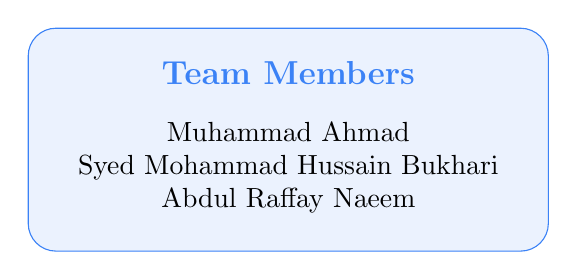
\begin{tikzpicture}
        \node[fill=primaryblue!10, draw=primaryblue, rounded corners=10pt, inner sep=12pt] {
            \begin{tabular}{c}
                {\large\bfseries\color{primaryblue} Team Members}\\[0.3cm]
                Muhammad Ahmad\\
                Syed Mohammad Hussain Bukhari\\
                Abdul Raffay Naeem
            \end{tabular}
        };
    \end{tikzpicture}
    
    \vspace{1cm}
    {\Large\bfseries\color{textdark} University of Central Punjab}\\
    {\color{textgray} Faculty of Information Technology | January 2026}
\end{center}
\end{titlepage}

\tableofcontents
\newpage

%%%%%%%%%%%%%%%%%%%%%%%%%%%%%%%%%%%%%%%%%%%%%%%%%%%%%%%%%%%%%%%
\section{User Research \& Validation}
%%%%%%%%%%%%%%%%%%%%%%%%%%%%%%%%%%%%%%%%%%%%%%%%%%%%%%%%%%%%%%%

\begin{questionbox}{What did you learn from talking to users?}
\end{questionbox}

We conducted a survey with \textbf{30+ UCP students} across multiple semesters (1st to 8th). Key findings:

\subsection{Survey Demographics}

\begin{center}
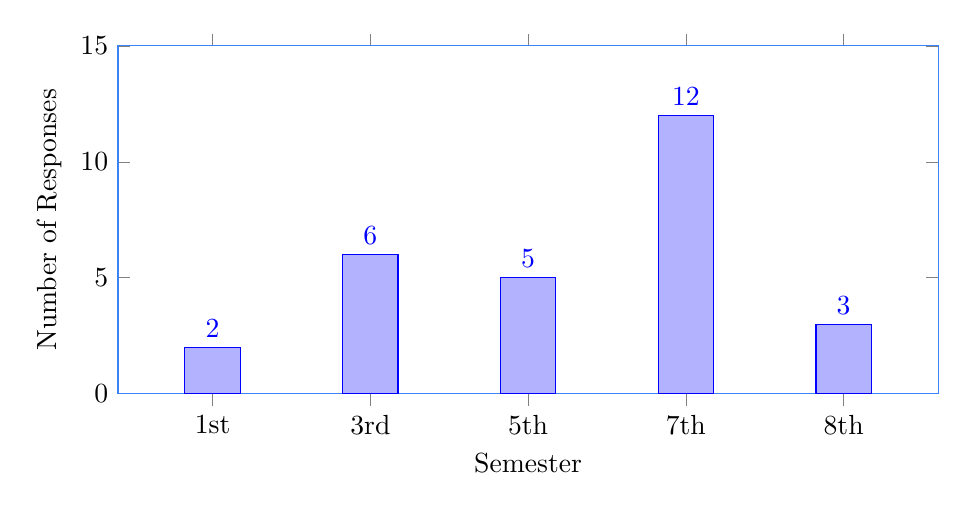
\begin{tikzpicture}
    \begin{axis}[
        ybar,
        width=12cm, height=6cm,
        bar width=20pt,
        ylabel={Number of Responses},
        xlabel={Semester},
        symbolic x coords={1st, 3rd, 5th, 7th, 8th},
        xtick=data,
        ymin=0, ymax=15,
        nodes near coords,
        nodes near coords align={vertical},
        fill=primaryblue!70,
        draw=primaryblue,
        enlarge x limits=0.15,
    ]
    \addplot coordinates {(1st, 2) (3rd, 6) (5th, 5) (7th, 12) (8th, 3)};
    \end{axis}
\end{tikzpicture}
\end{center}

\subsection{Key Finding 1: Registration Takes Too Long}

\begin{center}
\begin{tikzpicture}
    \pie[
        radius=3,
        color={dangerred!80, warningyellow!80, successgreen!60, primaryblue!50},
        text=legend,
        sum=auto
    ]{
        70/More than 45 min,
        15/30--45 min,
        12/15--30 min,
        3/Less than 15 min
    }
\end{tikzpicture}
\end{center}

\begin{insightbox}{\faIcon{lightbulb} Key Insight}
\textbf{70\% of students spend more than 45 minutes} on course registration each semester. This validates our core problem hypothesis.
\end{insightbox}

\subsection{Key Finding 2: Major Frustrations}

\begin{center}
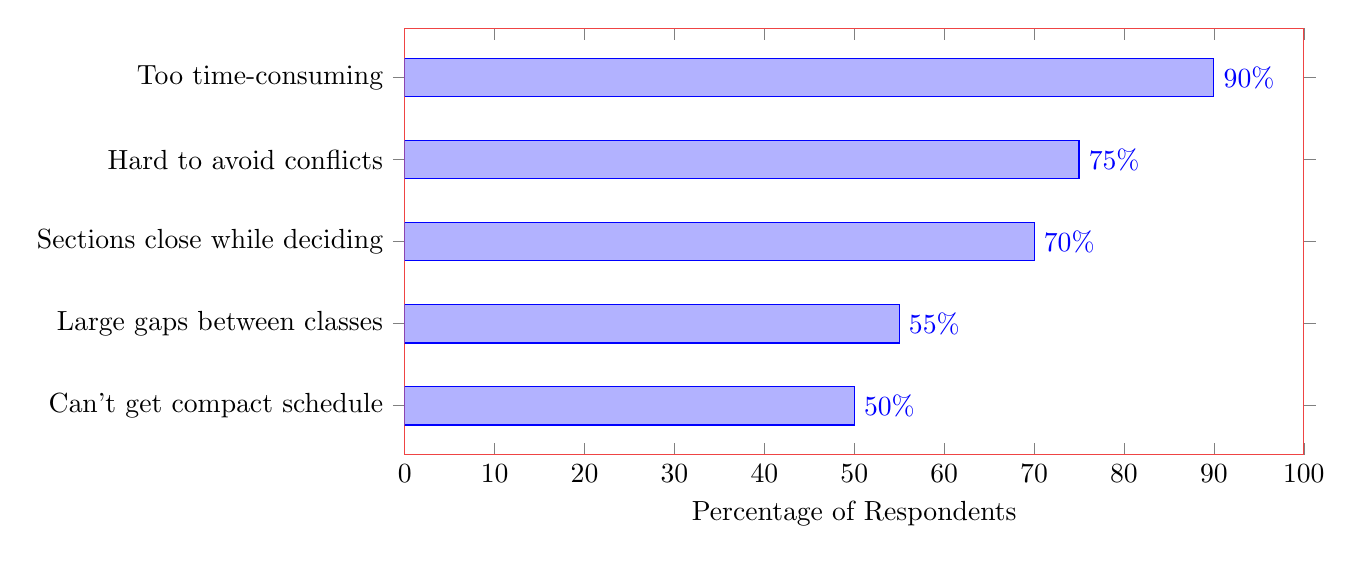
\begin{tikzpicture}
    \begin{axis}[
        xbar,
        width=13cm, height=7cm,
        bar width=14pt,
        xlabel={Percentage of Respondents},
        symbolic y coords={
            Can't get compact schedule,
            Large gaps between classes,
            Sections close while deciding,
            Hard to avoid conflicts,
            Too time-consuming
        },
        ytick=data,
        xmin=0, xmax=100,
        nodes near coords={\pgfmathprintnumber\pgfplotspointmeta\%},
        nodes near coords align={horizontal},
        fill=dangerred!70,
        draw=dangerred,
        enlarge y limits=0.15,
    ]
    \addplot coordinates {
        (90,Too time-consuming)
        (75,Hard to avoid conflicts)
        (70,Sections close while deciding)
        (55,Large gaps between classes)
        (50,Can't get compact schedule)
    };
    \end{axis}
\end{tikzpicture}
\end{center}

\textbf{Additional frustrations mentioned by students:}
\begin{itemize}[leftmargin=20pt]
    \item ``Portal server down'' / ``Portal dies again and again''
    \item ``Website crashes every 2 min''
    \item ``Registration comes in exam days''
    \item ``Sometimes sections are closed but portal shows available''
    \item ``Feels like booking tickets for a stadium that sells out immediately''
\end{itemize}

\subsection{Key Finding 3: Schedule Preferences}

\begin{center}
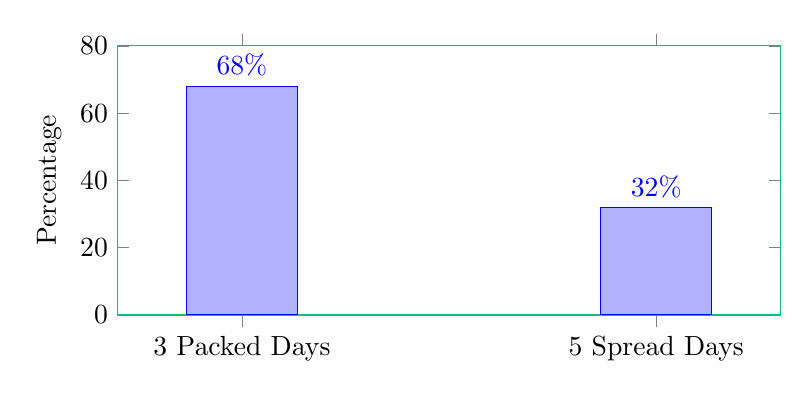
\begin{tikzpicture}
    \begin{axis}[
        ybar,
        width=10cm, height=5cm,
        bar width=40pt,
        ylabel={Percentage},
        symbolic x coords={3 Packed Days, 5 Spread Days},
        xtick=data,
        ymin=0, ymax=80,
        nodes near coords={\pgfmathprintnumber\pgfplotspointmeta\%},
        fill=successgreen!70,
        draw=successgreen,
        enlarge x limits=0.3,
    ]
    \addplot coordinates {(3 Packed Days, 68) (5 Spread Days, 32)};
    \end{axis}
\end{tikzpicture}
\end{center}

\begin{insightbox}{\faIcon{check-circle} Validated Assumption}
\textbf{68\% prefer 3 packed days} with back-to-back classes and minimal gaps. This confirms our optimization target.
\end{insightbox}

\subsection{Key Finding 4: Extension Adoption}

\begin{center}
\begin{tikzpicture}
    \pie[
        radius=2.5,
        color={successgreen!80, successgreen!50, textgray!40},
        text=legend,
        sum=auto
    ]{
        77/Definitely Yes,
        15/Probably Yes,
        8/Not Sure
    }
\end{tikzpicture}
\end{center}

\textbf{92\% of respondents expressed interest} in using a Chrome extension for automatic timetable optimization.

%%%%%%%%%%%%%%%%%%%%%%%%%%%%%%%%%%%%%%%%%%%%%%%%%%%%%%%%%%%%%%%
\newpage
\begin{questionbox}{How did user feedback change your solution design?}
\end{questionbox}

\begin{center}
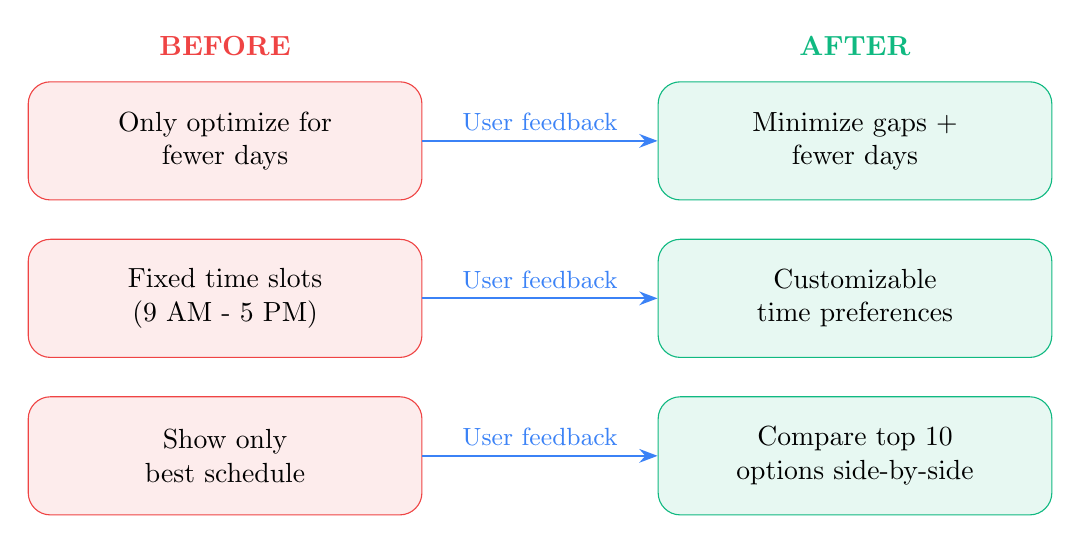
\begin{tikzpicture}[
    box/.style={rectangle, rounded corners=8pt, fill=white, draw=primaryblue, minimum width=5cm, minimum height=1.5cm, align=center},
    arrow/.style={-{Stealth}, thick, primaryblue}
]
    % Before
    \node[box, fill=dangerred!10, draw=dangerred] (b1) at (0, 4) {Only optimize for\\fewer days};
    \node[box, fill=dangerred!10, draw=dangerred] (b2) at (0, 2) {Fixed time slots\\(9 AM - 5 PM)};
    \node[box, fill=dangerred!10, draw=dangerred] (b3) at (0, 0) {Show only\\best schedule};
    
    % After
    \node[box, fill=successgreen!10, draw=successgreen] (a1) at (8, 4) {Minimize gaps +\\fewer days};
    \node[box, fill=successgreen!10, draw=successgreen] (a2) at (8, 2) {Customizable\\time preferences};
    \node[box, fill=successgreen!10, draw=successgreen] (a3) at (8, 0) {Compare top 10\\options side-by-side};
    
    % Arrows
    \draw[arrow] (b1) -- node[above, font=\small]{User feedback} (a1);
    \draw[arrow] (b2) -- node[above, font=\small]{User feedback} (a2);
    \draw[arrow] (b3) -- node[above, font=\small]{User feedback} (a3);
    
    % Labels
    \node[font=\bfseries\color{dangerred}] at (0, 5.2) {BEFORE};
    \node[font=\bfseries\color{successgreen}] at (8, 5.2) {AFTER};
\end{tikzpicture}
\end{center}

\textbf{Key Design Changes:}
\begin{enumerate}
    \item \textbf{Gap Minimization}: 55\% mentioned large gaps as frustration → Added gap detection
    \item \textbf{Time Filters}: Students prefer morning/afternoon slots → Added customizable time range
    \item \textbf{Side-by-Side Comparison}: Most requested feature (45\%) → Added visual comparison
    \item \textbf{Day Selection}: Allow preferred days → Added toggleable day chips
\end{enumerate}

%%%%%%%%%%%%%%%%%%%%%%%%%%%%%%%%%%%%%%%%%%%%%%%%%%%%%%%%%%%%%%%
\begin{questionbox}{Which assumptions were validated or disproved?}
\end{questionbox}

\begin{center}
\begin{tabular}{|p{5.5cm}|c|p{5cm}|}
\hline
\textbf{Assumption} & \textbf{Status} & \textbf{Evidence} \\
\hline
Registration takes too long & \cellcolor{successgreen!20}✓ Validated & 70\% spend 45+ minutes \\
\hline
Students want fewer campus days & \cellcolor{successgreen!20}✓ Validated & 68\% prefer 3-day schedule \\
\hline
All students face same issues & \cellcolor{warningyellow!20}Partially & Senior students (7th sem) more affected \\
\hline
Students will adopt extension & \cellcolor{successgreen!20}✓ Validated & 92\% interested \\
\hline
Time conflicts are main issue & \cellcolor{successgreen!20}✓ Validated & 75\% cited conflict avoidance \\
\hline
\end{tabular}
\end{center}

%%%%%%%%%%%%%%%%%%%%%%%%%%%%%%%%%%%%%%%%%%%%%%%%%%%%%%%%%%%%%%%
\newpage
\section{MVP Scope \& Features}
%%%%%%%%%%%%%%%%%%%%%%%%%%%%%%%%%%%%%%%%%%%%%%%%%%%%%%%%%%%%%%%

\begin{questionbox}{What core features will be included in the MVP?}
\end{questionbox}

\begin{center}
\begin{tikzpicture}[
    core/.style={rectangle, rounded corners=10pt, fill=successgreen!20, draw=successgreen, line width=2pt, minimum width=7cm, minimum height=1.2cm, align=center, font=\bfseries},
    support/.style={rectangle, rounded corners=8pt, fill=primaryblue!10, draw=primaryblue, minimum width=5.5cm, minimum height=1cm, align=center}
]
    % Core Features
    \node[font=\Large\bfseries\color{successgreen}] at (0, 5) {Core MVP Features};
    
    \node[core] (c1) at (0, 4) {\faIcon{search} Course Data Scraping from Portal};
    \node[core] (c2) at (0, 2.5) {\faIcon{cogs} Timetable Optimization Algorithm};
    \node[core] (c3) at (0, 1) {\faIcon{calendar-alt} Visual Timetable Display};
    \node[core] (c4) at (0, -0.5) {\faIcon{sliders-h} Day \& Time Preference Filters};
    
    % Connecting line
    \draw[successgreen, line width=3pt] (-4.5, 4) -- (-4.5, -0.5);
\end{tikzpicture}
\end{center}

\begin{questionbox}{Which features are out of scope for this hackathon?}
\end{questionbox}

\begin{center}
\begin{tikzpicture}[
    scope/.style={rectangle, rounded corners=5pt, fill=dangerred!10, draw=dangerred, minimum width=5cm, minimum height=0.8cm, align=center}
]
    \node[scope] at (0, 0) {\faIcon{times} One-click auto-enrollment};
    \node[scope] at (0, -1) {\faIcon{times} Waitlist notifications};
    \node[scope] at (0, -2) {\faIcon{times} Multi-semester planning};
    \node[scope] at (0, -3) {\faIcon{times} Mobile app version};
\end{tikzpicture}
\end{center}

\begin{questionbox}{How will your MVP demonstrate value to users?}
\end{questionbox}

\begin{featurebox}
\textbf{Value Demonstration:}
\begin{itemize}
    \item \textbf{Time Savings}: 45+ minutes → Under 5 minutes (90\% reduction)
    \item \textbf{Optimal Schedules}: Guaranteed 3-day timetables when possible
    \item \textbf{Conflict-Free}: Zero scheduling conflicts
    \item \textbf{Visual Comparison}: See top 10 options ranked by score
\end{itemize}
\end{featurebox}

%%%%%%%%%%%%%%%%%%%%%%%%%%%%%%%%%%%%%%%%%%%%%%%%%%%%%%%%%%%%%%%
\section{Implementation \& Technical Planning}
%%%%%%%%%%%%%%%%%%%%%%%%%%%%%%%%%%%%%%%%%%%%%%%%%%%%%%%%%%%%%%%

\begin{questionbox}{Which technical tools, platforms, or languages will you use?}
\end{questionbox}

\begin{center}

\begin{tikzpicture}[
    tech/.style={rectangle, rounded corners=8pt, fill=textdark, text=white, minimum width=3cm, minimum height=1.2cm, align=center, font=\small\bfseries}
]
    \node[tech] (t1) at (0, 0) {Manifest V3\\Chrome Extension};
    \node[tech] (t2) at (4, 0) {JavaScript\\Vanilla JS};
    \node[tech] (t3) at (8, 0) {HTML/CSS\\Popup UI};
    \node[tech] (t4) at (12, 0) {DOM Scraping\\Content Script};
    
    \draw[-{Stealth}, thick, primaryblue] (t1) -- (t2);
    \draw[-{Stealth}, thick, primaryblue] (t2) -- (t3);
    \draw[-{Stealth}, thick, primaryblue] (t3) -- (t4);
\end{tikzpicture}
\end{center}

\begin{questionbox}{How will you prioritize features for Day 2 development?}
\end{questionbox}

\begin{center}
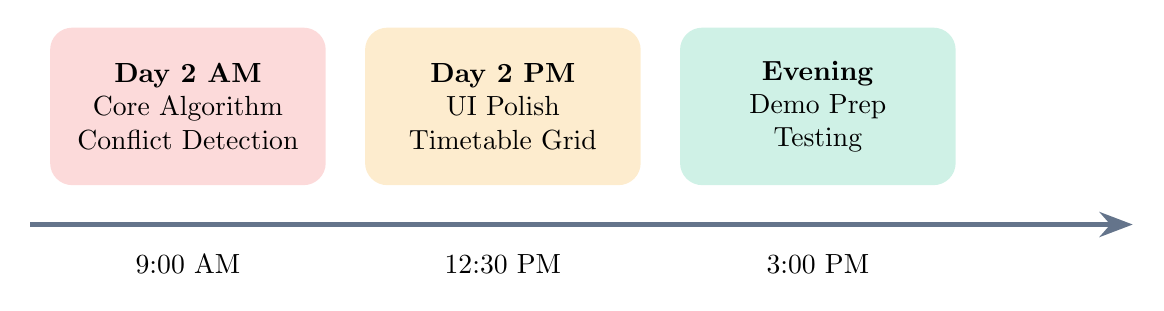
\begin{tikzpicture}[
    phase/.style={rectangle, rounded corners=8pt, minimum width=3.5cm, minimum height=2cm, align=center}
]
    % Timeline
    \draw[-{Stealth}, line width=2pt, textgray] (0, 0) -- (14, 0);
    
    % Phases
    \node[phase, fill=dangerred!20] at (2, 1.5) {\textbf{Day 2 AM}\\Core Algorithm\\Conflict Detection};
    \node[phase, fill=warningyellow!20] at (6, 1.5) {\textbf{Day 2 PM}\\UI Polish\\Timetable Grid};
    \node[phase, fill=successgreen!20] at (10, 1.5) {\textbf{Evening}\\Demo Prep\\Testing};
    
    % Time markers
    \node at (2, -0.5) {9:00 AM};
    \node at (6, -0.5) {12:30 PM};
    \node at (10, -0.5) {3:00 PM};
\end{tikzpicture}
\end{center}

\begin{questionbox}{What challenges do you anticipate, and how will you address them?}
\end{questionbox}

\begin{center}
\begin{tabular}{|p{4.5cm}|p{6cm}|}
\hline
\textbf{Challenge} & \textbf{Solution} \\
\hline
Too many combinations crash & Limit to 50,000 combinations; auto-reduce sections \\
\hline
Portal DOM changes & Use flexible selectors; add data attributes \\
\hline
Courses don't fit filters & Show warning; allow exclusion \\
\hline
Time conflicts complex & Interval overlap algorithm \\
\hline
\end{tabular}
\end{center}

%%%%%%%%%%%%%%%%%%%%%%%%%%%%%%%%%%%%%%%%%%%%%%%%%%%%%%%%%%%%%%%
\section{Day 1 Deliverables Summary}
%%%%%%%%%%%%%%%%%%%%%%%%%%%%%%%%%%%%%%%%%%%%%%%%%%%%%%%%%%%%%%%

\begin{center}
\begin{tikzpicture}[
    check/.style={rectangle, rounded corners=8pt, fill=successgreen!10, draw=successgreen, minimum width=13cm, minimum height=1cm, align=left}
]
    \node[check] at (0, 3) {\color{successgreen}\faIcon{check-circle} \textbf{Refined Problem Statement}: 70\% students waste 45+ min on registration};
    \node[check] at (0, 1.8) {\color{successgreen}\faIcon{check-circle} \textbf{Clearly Defined MVP Scope}: 4 core features, visual timetable, filters};
    \node[check] at (0, 0.6) {\color{successgreen}\faIcon{check-circle} \textbf{Evidence of User Research}: 30+ survey responses analyzed};
    \node[check] at (0, -0.6) {\color{successgreen}\faIcon{check-circle} \textbf{Initial Working Components}: Extension structure, DOM scraper, popup UI};
    \node[check] at (0, -1.8) {\color{successgreen}\faIcon{check-circle} \textbf{Repository Setup}: GitHub repo with README, organized structure};
\end{tikzpicture}
\end{center}

\end{document}
